\documentclass[9pt,twocolumn,twoside]{Gunadarma}
\setboolean{shortarticle}{false}


\title{\begin{center}
		\textit{Drone Monitoring} dan \textit{Management System}
	\end{center}}

\author[1]{Candra Gunawan}
\affil[1]{Magister Manajement Sistem Informasi, Universitas Gunadarma, 2016, Jakarta}
\affil[1]{Corresponding author: cgunawan@tibco.com}

\author[2]{Deny Pratama}
\affil[2]{Magister Manajement Sistem Informasi, Universitas Gunadarma, 2016, Jakarta}
\affil[2]{Corresponding author: denyuno@gmail.com}

\author[3]{Dewi Apriyani}
\affil[3]{Magister Manajement Sistem Informasi, Universitas Gunadarma, 2016, Jakarta}
\affil[3]{Corresponding author: uwiart93@gmail.com}

\author[4]{Putri Sari Sigiro}
\affil[4]{Magister Manajement Sistem Informasi, Universitas Gunadarma, 2016, Jakarta}
\affil[4]{Corresponding author: putri.sigiro@gmail.com}

\author[5]{Anesia Puji Kinanti}
\affil[5]{Magister Manajement Sistem Informasi, Universitas Gunadarma, 2016, Jakarta}
\affil[5]{Corresponding author: Anesiaakinanti@gmail.com}

\dates{Compiled using \LaTeX\ \today}


\ociscodes{}

\doi{\url{http://Gunadarma.ac.id}}

\begin{abstract}
\textit{Drone}  merupakan pesawat nir awak, atau pesawat tanpa awak. Pesawat ini tidak membutuhkan seorang pilot untuk memandu nya. Bentuknya bermacam - macam mengikuti tujuan utama penggunaan. Sedangkan cara kerja \textit{drone} yaitu memanfaatkan kendali jarak jauh atau sistem remote dimana \textit{pilot} memegang kontrol dari darat. Dengan semakin berkembang nya \textit{drone}, dan semakin banyak nya pilot \textit{drone} untuk berbagai macam keperluan, seperti misal untuk hobi maupun komersil, maka penulis berpikir diperlukan suatu sistem manajemen dan deteksi \textit{drone}. Tujuan nya adalah, agar \textit{Drone} yang saat ini bisa terpantau dan bisa diketahui rute penerbangan nya. Dengan begitu, maka \textit{drone} akan semakin ter-\textit{manage}.  


\end{abstract}

\setboolean{displaycopyright}{true}

\begin{document}

\maketitle
\thispagestyle{fancy}
\ifthenelse{\boolean{shortarticle}}{\abscontent}{}

\section{Pendahuluan}
\subsection{Latar Belakang Masalah}


\textit{Drone} merupakan pesawat nir awak atau pesawat tanpa awak. Pesawat ini tidak membutuhkan seorang pilot untuk memandunya, serta sering disebut sebagai pesawat \textit{UAV} atau Unmanned\textit{ Aerial Vehicle}. Sebagai pesawat tak berawak, tentunya tidak ada manusiapun di dalam sebuah drone. Bentuknya bermacam-macam mengikuti tujuan utama penggunaan. Sedangkan cara kerja drone yaitu memanfaatkan kendali jarak jauh atau sistem remote dimana pilote memegang kontrol dari darat. Dengan semakin berkembangnya teknologi, kini adapula drone yang memiliki kemampuan untuk mengendalikan dirinya secara mandiri setelah diprogram menggunakan komputer onboard yang dipasangkan di drone itu sendiri.

Pada awalnya, pesawat jenis drone digunakan sebagai alat pengintaian dan penyerangan atau secara umum dimanfaatkan oleh pihak militer. Namun, dewasa ini pemanfaatan teknologi drone juga menjalar ke area sipil (non-militer). Sampai saat ini, drone telah dimanfaatkan pula dalam industri bisnis dan diaplikasikan ke dalam berbagai layanan, seperti:


\begin{itemize}
	\item Pengiriman komersil
	\item Pengawasan keamanan komersil
	\item Eksplorasi tambang, minyak dan mineral
	\item Bantuan kesehatan darurat
	\item ProsesPembuatan film
\end{itemize}


Dengan semakin berkembangnya teknologi, semakin banyak pengguna \textit{Drone}, baik untuk komersial maupun Non-komersial. Juga, banyak nya berbagai spesifikasi \textit{Drone}, mulai dari kecepatan rendah, kecepatan tinggi, ketinggian rendah bahkan ada yang bisa mencapai ketinggian tertentu. Dengan muncul berbagai jenis \textit{Drone} tersebut, maka keberadaan \textit{Drone} yang sebelumnya bermanfaat bisa menimbulkan resiko. Salah satu resiko nya adalah mengganggu penerbangan pesawat komersial.

Untuk me-minimalisir resiko tersebut, maka penulis mengusulkan untuk dibuatnya \textit{Drone Management System}. Tujuannya adalah agar \textit{Drone} yang saat ini ada, bisa \textit{manage}. Tugas dari sistem ini adalah membuat Drone bisa di monitor, dan bisa di identifikasi. Agar nanti nya adalah penggunaan \textit{Drone} bisa di pertanggungjawabkan. 

\subsection{Rumusan Masalah}
Rumusan masalah pada jurnal \textbf{"Penggunaan Aplikasi \textit{Selenium} Untuk \textit{Automatic Testing} Pada Metodologi \textit{DevOps}"} adalah untuk menjelasakan bagaimana implementasi \textit{automated testing} dengan menggunakan \textit{tool selenium}  dan kaitan nya dengan metodologi \textit{DevOps}. 


\subsection{Tujuan Penulisan}
Tujuan penulisan ini adalah untuk membuat analisa dan rancangan suatu \textit{Drone Management System} dan bagaimana penerapan juga manfaat nya terhadap masyarakat.  


\section{Landasan Teori}

\subsection{Cara Kerja Drone}
Sebuah pesawat tak berawak yang khas terbuat dari bahan komposit ringan untuk mengurangi berat badan dan meningkatkan kemampuan manuver. kekuatan material komposit ini memungkinkan drone militer untuk pelayaran pada ketinggian yang sangat tinggi. Drone dilengkapi dengan keadaan yang berbeda dari teknologi seni seperti infra-merah kamera (\textit{UAV} militer), \textit{GPS} dan laser (\textit{UAV} militer). Drone dapat dikontrol oleh sistem kontrol jarak jauh atau kokpit tanah. Drone datang dalam berbagai ukuran, dengan pesawat tak berawak besar sebagian besar digunakan untuk tujuan militer seperti pesawat tak berawak Predator, drone kecil lainnya yang dapat diluncurkan dengan tangan, untuk pesawat tak berawak lainnya yang membutuhkan landasan pacu pendek. Sebuah sistem kendaraan udara tak berawak memiliki dua bagian, pesawat tak berawak itu sendiri dan sistem kontrol.

\begin{figure}[htbp]
	\begin{center}
		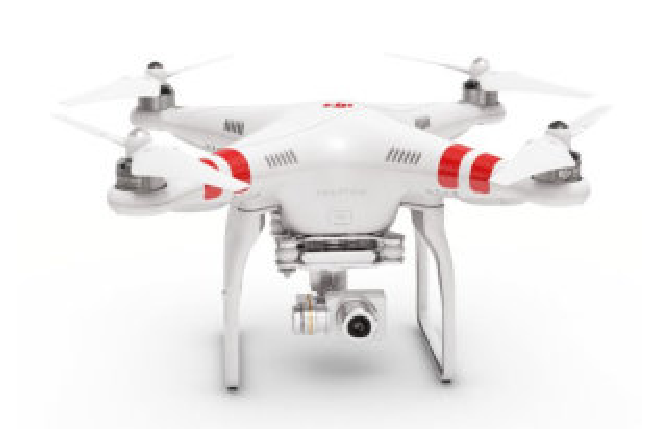
\includegraphics[width=1\columnwidth]{drone.eps} \label{fig:1-noFCase1}
	\end{center}
	\caption{Drone}
\end{figure}

Sampai saat ini, drone telah dimanfaatkan pula dalam industri bisnis dan diaplikasikan ke dalam berbagai layanan, seperti:
\begin{itemize}
	\item Pengiriman komersil
	\item Pengawasan keamanan komersil
	\item Eksplorasi tambang, minyak dan mineral
	\item Bantuan kesehatan darurat
	\item ProsesPembuatan film
\end{itemize}
Semakin canggih teknologi yang ditanam dalam suatu desainnya, semakin rumit pula cara kerja drone. Namun, kemudahan mengatur pesawat tanpa awak ini secara jarak jauh justru memberikan fleksibilitas bagi pengguna melakukan suatu misi di area tertentu atau tidak mudah dijangkau oleh manusia.

Drone sendiri dalam praktik nya terdiri atas beberapa komponen, yaitu :
\begin{itemize}
	\item \textit{Flight Control Board}, yang berfungsi sebagai otak dari drone tersebut. 
	\item \textit{Frame} atau kerangka dari drone
	\item \textit{Motor}
	\item \textit{Electronic Speed Control} (ESC), yaitu untuk mengatur kecepatan drone
	\item Propeller (Baling-baling)
	\item Baterai dan charger
	\item \textit{Remote Control} untuk mengendalikan Drone
\end{itemize}


\subsection{Cara Kerja Radar}
Radar (yang dalam bahasa Inggris merupakan singkatan dari \textit{Radio Detection and Ranging}, yang berarti deteksi dan penjarakan radio) adalah suatu sistem gelombang elektromagnetik yang berguna untuk mendeteksi, mengukur jarak dan membuat map benda-benda seperti pesawat terbang, berbagai kendaraan bermotor dan informasi cuaca (hujan). Panjang gelombang yang dipancarkan radar bervariasi mulai dari milimeter hingga meter. Gelombang radio/sinyal yang dipancarkan dan dipantulkan dari suatu benda tertentu akan ditangkap oleh radar. Dengan menganalisis sinyal yang dipantulkan tersebut, pemantul sinyal dapat ditentukan lokasinya dan melalui analisis lebih lanjut dari sinyal yang dipantulkan dapat juga ditentukan jenisnya. Meskipun sinyal yang diterima relatif lemah/kecil, namun radio sinyal tersebut dapat dideteksi dan diperkuat oleh penerima radar.


\begin{figure}[htbp]
\begin{center}
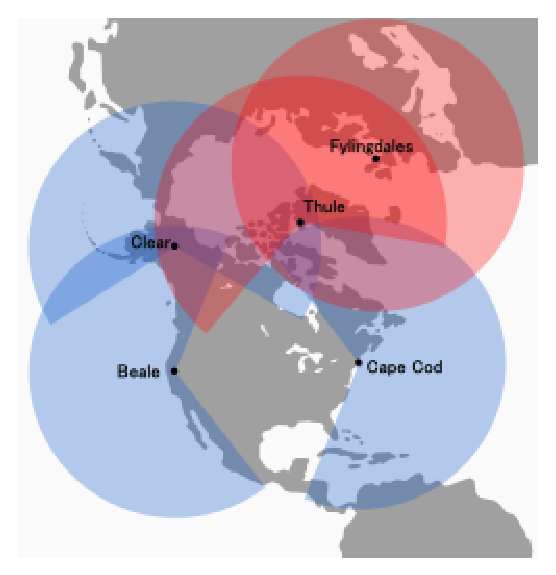
\includegraphics[width=1\columnwidth]{radar.eps} \label{fig:1-noFCase1}
\end{center}
\caption{Radar Range Area}
\end{figure}

Ada tiga komponen utama yang tersusun di dalam sistem radar, yaitu antena, transmitter (pemancar sinyal) dan receiver (penerima sinyal).
\subsubsection{Antena}
Antena yang terletak pada radar merupakan suatu antena reflektor berbentuk piring parabola yang menyebarkan energi elektromagnetik dari titik fokusnya dan dipantulkan melalui permukaan yang berbentuk parabola. Antena radar memiliki du akutub (dwikutub). Input sinyal yang masuk dijabarkan dalam bentuk \textit{phased-array} (bertingkat atau bertahap). Ini merupakan sebaran unsur-unsur objek yang tertangkap antena dan kemudian diteruskan ke pusat sistem RADAR.

\subsubsection{Penerima sinyal (receiver)}
Pada sistem radar, penerima sinyal (receiver) berfungsi sebagai penerima kembali pantulan gelombang elektromagnetik dari sinyal objek yang tertangkap oleh radar melalui reflektor antena. Pada umumnya, receiver memiliki kemampuan untuk menyaring sinyal yang diterimanya agar sesuai dengan pendeteksian yang diinginkan, dapat memperkuat sinyal objek yang lemah dan meneruskan sinyal objek tersebut ke pemroses data dan sinyal (signal and data processor), dan kemudian menampilkan gambarnya di layar monitor (display). Selain tiga komponen di atas, sistem radar juga terdiri dari beberapa komponen pendukung lainnya, yaitu

\begin{itemize}
	\item \textit{Waveguide}, berfungsi sebagai penghubung antara antena dan transmitter. 
	\item \textit{Duplexer},  berfungsi sebagai tempat pertukaran atau peralihan antara antena dan penerima atau pemancar sinyal ketika antena digunakan dalam kedua situasi tersebut.
	\item \textit{Software}, merupakan suatu bagian elektronik yang berfungsi mengontrol kerja seluruh perangkat dan antena ketika melakukan tugasnya masing-masing.

\end{itemize}

Dalam bidang penerbangan, penggunaan radar terlihat jelas pada pemakaian \textit{Air Traffic Control} (ATC). \textit{Air Traffic Control} merupakan suatu kendali dalam pengaturan lalu lintas udara. Tugasnya adalah untuk mengatur lalu lalang serta kelancaran lalu lintas udara bagi setiap pesawat terbang yang akan lepas landas (\textit{take off}), terbang di udara, maupun yang akan mendarat (\textit{landing}). ATC juga berfungsi untuk memberikan layanan bantuan informasi bagi pilot tentang cuaca, situasi dan kondisi bandara yang dituju. radar mempunyai kelebihan dalam komunikasi . radar yang sangat kuat dapat membantu pilot untuk melihat cuaca , layaknya pesawat terbang dan lain lain


\subsection{Transponder}

transponder pertamakali dibuat ketika World war 2 berlangsung yang dikembangkan oleh inggris dan amerika serikat sebagai "Identification Friend Or Foe" (IFF) yang fungsinya mendeteksi pesawat ini asalnya dari musuh atau bukan menggunakan kode-kode tertentu.

\subsubsection{jenis Jenis Transponder Mode}
\begin{enumerate}
	\item Mode C, Mode ini mentransmit keseluruhan data dari ketinggian, nomor penerbangan, jenis pesawat, dan lain-lain.
	\item Mode S, transponder ini mentransmit data yang sama seperti Mode C namun dilengkapi dengan pemancar ADS-B yang mana merupakan teknologi radar terbaru yang lebih akurat.
	\item Mode X, Tidak Memancarkan Jenis Pesawat, dan Ketinggian
	\item Mode P, Ketinggian di transmit namun identitas pesawat tidak di transmit
	\item Mode I, Ketinggian di transmit namun identitas pesawat di transmit
	\item Mode N, pesawat tanpa transponder, biasanya pesawat \textit{ultralight}.
\end{enumerate}


\section{Pembahasan}

\subsection{\textit{Monitoring Drone}}

Drone saat ini digunakan baik untuk tujuan komersial maupun Non-Komersial. Tapi, dengan semakin berkembang nya zaman, maka keberadaan Drone, yang awal nya memberikan manfaat, menjadi perlu suatu pengawasan. Karena Drone saat ini tidak ada pengawasan, jadi bisa memasuki daerah - daerah terlarang, dan bisa menjadi berbahaya. 

Sebagai contoh kasus, Drone yang dilengkapi kamera, jika di terbangkan ke area militer tanpa ada nya pengawasan, bisa membocorkan data wilayah militer, dan bisa jadi ke depan nya membahayakan keamanan nasional. Begitu juga jika terjadi Drone diterbangkan di dekat lintasan pesawat, maka bisa mengganggu lalu lintas pesawat, dan otomatis bisa mengganggu penerbangan pesawat. 

Karena itu, perlu ada nya monitoring Drone. Drone bisa saja di monitor dan di identifikasi, tapi tentu nya harus dimasukkan ke dalam standar pembuatan Drone itu sendiri. Dengan mengacu kepada teori sebelum nya, agar Drone bisa terlihat posisi, ketinggian dan juga identitas nya, perlu di buat suatu teknologi di dalam standar Drone nya tersebut, dengan memanfaatkan teknologi \textit{transponder}. 

untuk system pengawasan nya sendiri, agar bisa melacak transponder tersebut maka meng-adaptasi teknologi \textit{radar}. Dengan teknologi ini, maka dimungkinkan untuk mengawasi dan meng-identifikasi setiap drone yang digunakan. Teknologi ini lebih masuk akal, karena pada dasar nya menggunakan teknologi yang sudah ada dan dapat di handalkan. 
\\ \\ \\ \\ \\ \\ \\ \\ \\ \\ \\ \\ \\ \\ \\ \\
\\ \\ \\ \\ \\ \\ \\ \\ \\ \\ \\ \\ 

\subsection{Analysis Penggunaan Transponder dan Sistem Radar}

Salah satu komponen yang terdapat pada Drone adalah \textit{Flight Control Board}. Saat ini, banyak sekali FCB dengan berbagai kemampuan di dalamnya. Fitur yang biasa ada di FCB seperti misal nya adalah \textit{Gyro, GPS, Accelerometer, magnometer} dan sebagai nya. Dan tidak menutup kemungkinan di dalam FCB ini ditambahkan fitur lain.

Salah satu ide untuk monitor Drone adalah dengan menanamkan transponder di dalam FCB ini. Sehingga nantinya saat terbang, Drone akan mengirimkan sinyal, sehingga bisa di deteksi dan di identifikasi drone tersebut dari darat. 

\begin{figure}[htbp]
	\begin{center}
		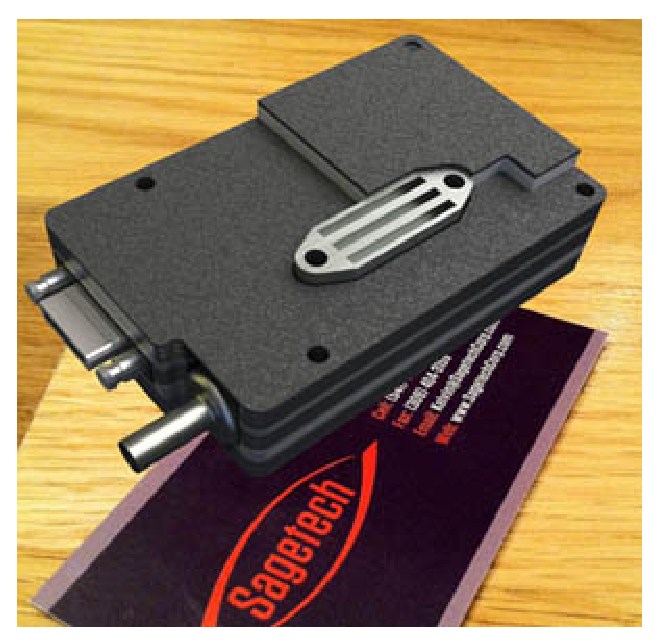
\includegraphics[width=1\columnwidth]{transponder.eps} \label{fig:1-noFCase1}
	\end{center}
	\caption{Mini Transponder}
\end{figure}


Fitur ini mulai di sematkan oleh beberapa perusahaan besar yang mulai menggunakan drone sebagai salah satu inovasi dan lini bisnis nya. Salah satu nya adalah google. Google mulai mem-produksi mini \textit{transponder} untuk disematkan di drone. Nantinya \textit{mini transponder} ini akan \textit{compatible} dengan semua drone yang ada di pasaran. 


\begin{figure}[htbp]
	\begin{center}
		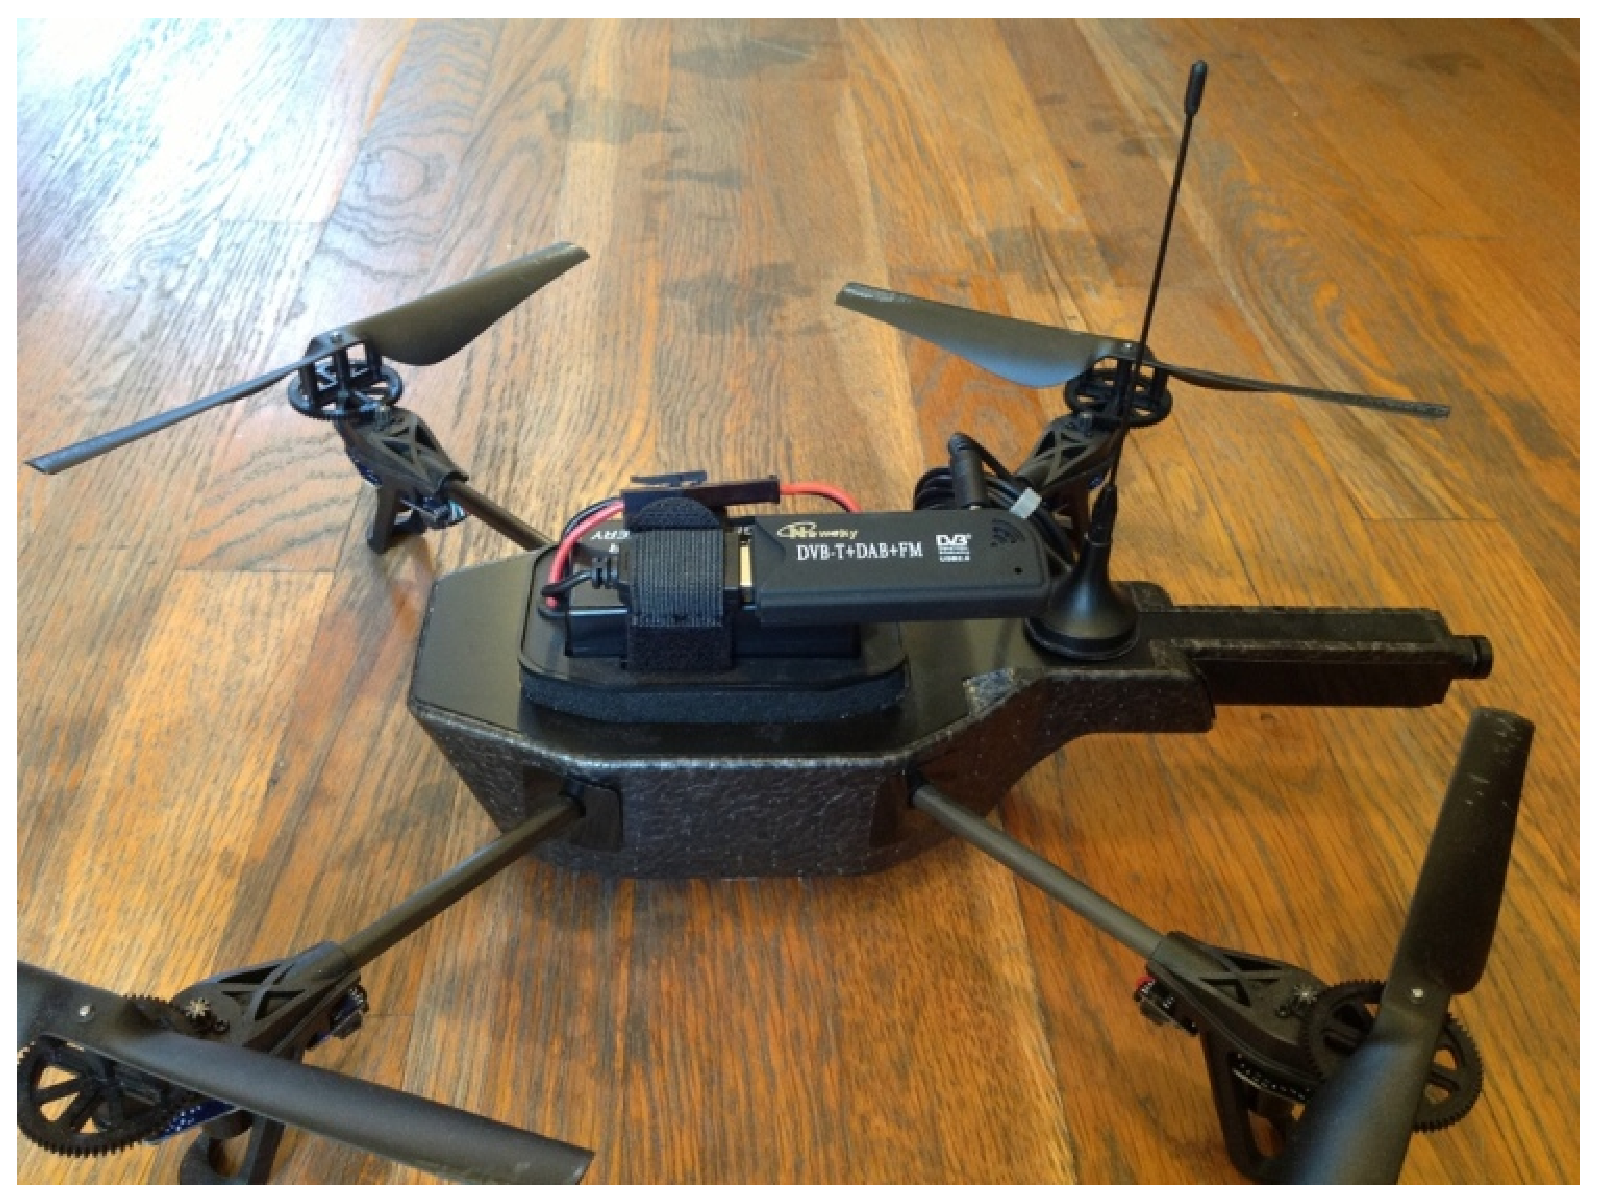
\includegraphics[width=1\columnwidth]{DroneWithTransponder.eps} \label{fig:1-noFCase1}
	\end{center}
	\caption{Drone With Mini Transponder}
\end{figure}


Setelah itu, perlu dibuat standar baku dalam identifikasi drone. Dan juga fasilitas radar yang mumpuni yang bisa men-deteksi drone dengan \textit{transponder} ini dalam radius tertentu. 



\section{Kesimpulan}
\subsection{Rangkuman}

Drone saat ini sudah digunakan banyak, baik untuk tujuan komersial maupun non-komersial. Komersial, seperti misal nya mulai digunakan untuk mengirim barang, sebagai monitoring lingkungan ataupun sekedar sebagai pemancar signal. Untuk tujuan non-komrsial, drone pun digunakan seperti misalnya untuk bermain, ataupun hanya sekedar hobi. Dengan meningkatnya penggunaan drone, maka terdapat resiko jika drone tersebut disalahgunakan, ataupun memasuki kawasan - kawasan sensitif, seperti misal nya bandara ataupun pangkalan militer. Maka perlu dibuat mekanisime deteksi dan identifikasi Drone. Salah satu cara deteksi adalah dengan menggunakan radar. Untuk identifikasi, maka diperlukan perangkat yang bisa \textit{compatible} dengan system radar. Salah satu alat tersebut adalah transponder. Dan Penulis menyarankan untuk transponder ini dibenamkan sebagai salah satu fitur di FCB drone tersebut. 


\subsection{Saran}
Adapun dari penulisan berikut ini, ada beberapa saran yang penulis rangkum di dalam penulisan ini :
\begin{itemize}
\item Penulis baru menggambarkan secara teori penggunaan transponder 
\item Penulis belum bisa menjabarkan secara detail proses identifikasi di transponder
\item Penulis belum menggambarkan tentang tata cara instalasi transponder tersebut. 
\end{itemize}

\section{Daftar Pustaka}


%\bigskip \noindent See \href{link}{Supplement 1} for supporting content.

%\noindent Add citations manually or use BibTeX. See \cite{Zhang:14}.
%\noindent Add citations manually or use BibTeX. See \cite{Agile:01}.
% Bibliography

%\bibliography{sample}

%Manual citation list
%\begin{thebibliography}{1}
%\bibitem{Zhang:14}
%Y.~Zhang, S.~Qiao, L.~Sun, Q.~W. Shi, W.~Huang, %L.~Li, and Z.~Yang,
% \enquote{Photoinduced active terahertz metamaterials with nanostructured
%vanadium dioxide film deposited by sol-gel method,} Opt. Express \textbf{22},
%11070--11078 (2014).
%\end{thebibliography}

\end{document}